%%%%%%%%%%%%%%%%%%%%%%%%%%%%%%%%%%%%%%%%%%%%%%%%%%%%%%%%%%%%%%%%%%%%
%% I, the copyright holder of this work, release this work into the
%% public domain. This applies worldwide. In some countries this may
%% not be legally possible; if so: i~grant anyone the right to use
%% this work for any purpose, without any conditions, unless such
%% conditions are required by law.
%%%%%%%%%%%%%%%%%%%%%%%%%%%%%%%%%%%%%%%%%%%%%%%%%%%%%%%%%%%%%%%%%%%%

\documentclass[
  digital,     %% The `digital` option enables the default options for the
               %% digital version of a~document. Replace with `printed`
               %% to enable the default options for the printed version
               %% of a~document.
%%  color,       %% Uncomment these lines (by removing the %% at the
%%               %% beginning) to use color in the printed version of your
%%               %% document
  oneside,     %% The `oneside` option enables one-sided typesetting,
               %% which is preferred if you are only going to submit a
               %% digital version of your thesis. Replace with `twoside`
               %% for double-sided typesetting if you are planning to
               %% also print your thesis. For double-sided typesetting,
               %% use at least 120 g/m² paper to prevent show-through.
  nosansbold,  %% The `nosansbold` option prevents the use of the
               %% sans-serif type face for bold text. Replace with
               %% `sansbold` to use sans-serif type face for bold text.
  colorbold, %% The `nocolorbold` option disables the usage of the
               %% blue color for bold text, instead using black. Replace
               %% with `colorbold` to use blue for bold text.
  lof,         %% The `lof` option prints the List of Figures. Replace
               %% with `nolof` to hide the List of Figures.
  nolot,         %% The `lot` option prints the List of Tables. Replace
               %% with `nolot` to hide the List of Tables.
]{fithesis4}
%% The following section sets up the locales used in the thesis.
\usepackage[resetfonts]{cmap} %% We need to load the T2A font encoding
\usepackage[T1,T2A]{fontenc}  %% to use the Cyrillic fonts with Russian texts.
\usepackage[
  main=czech, %% By using `czech` or `slovak` as the main locale
                %% instead of `english`, you can typeset the thesis
                %% in either Czech or Slovak, respectively.
  english, german, czech, slovak %% The additional keys allow
]{babel}        %% foreign texts to be typeset as follows:
%%
%%   \begin{otherlanguage}{german}  ... \end{otherlanguage}
%%   \begin{otherlanguage}{russian} ... \end{otherlanguage}
%%   \begin{otherlanguage}{czech}   ... \end{otherlanguage}
%%   \begin{otherlanguage}{slovak}  ... \end{otherlanguage}
%%
%% For non-Latin scripts, it may be necessary to load additional
%% fonts:
\usepackage{paratype}
\def\textrussian#1{{\usefont{T2A}{PTSerif-TLF}{m}{rm}#1}}
%%
%% The following section sets up the metadata of the thesis.
\thesissetup{
    date        = \the\year/\the\month/\the\day,
    university  = mu,
    faculty     = fi,
    type        = bc,
    department  = Katedra počítačových systémů a~komunikací,
    author      = Denisa Maťátková,
    advisor     = {doc. Ing. RNDr. Barbora Bühnová, Ph.D.},
    title       = {Výuka programování na střední škole s~využitím micro:bit},
    TeXtitle    = {Výuka programování na střední škole s~využitím micro:bit},
    keywords    = {Micro:bit, Nezha, MicroPython (Python), algoritmizace, výuka, programování na SŠ, RVP, výukové materiály},
    TeXkeywords = {Micro:bit, Nezha, MicroPython (Python), algoritmizace, výuka, programování na SŠ, RVP, výukové materiály, \ldots},
    abstract    = {Cílem této práce bylo představit platformu micro:bit jako prostředek pro výuku algoritmizace na středních školách v~kontextu revidovaného RVP G pro oblast informatiky. Na základě získaných znalostí vytvořit a~zrealizovat sadu úloh s~využitím vybrané sady. Vytvořené úlohy jsou součástí deseti kompletních lekcí, které pokrývají oblast algoritmizace a~programování z~revidovaného RVP a~jsou doplněny o~metodické pokyny pro učitele. Na vytvořených úlohách si žáci osvojí základní programovací koncepty a~návrh algoritmů s~využitím programovacího jazyka MicroPython.},
    thanks      = {Děkuji},
    bib         = example.bib,
    %% Remove the following line to use the JVS 2018 faculty logo.
    %facultyLogo = fithesis-fi,
}
\usepackage{makeidx}      %% The `makeidx` package contains
\makeindex                %% helper commands for index typesetting.
%% These additional packages are used within the document:
\usepackage{paralist} %% Compact list environments
\usepackage{comment}
\usepackage{amsmath}  %% Mathematics
\usepackage{amsthm}
\usepackage{amsfonts}
\usepackage{url}      %% Hyperlinks
\usepackage{markdown} %% Lightweight markup
\usepackage{listings} %% Source code highlighting
\lstset{
  basicstyle      = \ttfamily,
  identifierstyle = \color{black},
  keywordstyle    = \color{blue},
  keywordstyle    = {[2]\color{cyan}},
  keywordstyle    = {[3]\color{olive}},
  stringstyle     = \color{teal},
  commentstyle    = \itshape\color{magenta},
  breaklines      = true,
  captionpos      = b,
  numbers         = left,
  numberstyle     = \scriptsize,
  xleftmargin     = 2em
}

\renewcommand{\lstlistingname}{Python kód}% Listing -> Algorithm
\renewcommand{\lstlistlistingname}{Seznam \lstlistingname ů}% List of Listings -> List of Algorithms

\usepackage{microtype}
\microtypesetup{nopatch=item}

\usepackage{floatrow} %% Putting captions above tables
\floatsetup[table]{capposition=top}
\usepackage[babel]{csquotes} %% Context-sensitive quotation marks

\begin{document}
%% The \chapter* command can be used to produce unnumbered chapters:

\chapter{Úvod}
%% Unlike \chapter, \chapter* does not update the headings and does not
%% enter the chapter to the table of contents. i~we want correct
%% headings and a~table of contents entry, we must add them manually:

%\markright{\textsc{Úvod}}
%\addcontentsline{toc}{chapter}{Úvod}
V současné době se programování stává důležitým nástrojem pro rozvoj kreativity, logického myšlení a~analytických schopností.  Je tedy nezbytné, aby byly vytvořeny vhodné výukové materiály, které v kombinaci s vhodnými prostředky žákům umožní osvojit si tyto dovednosti efektivně.

Cílem této práce je představit platformu micro:bit jako prostředek pro výuku algoritmizace na středních školách v~kontextu revidovaného rámcového vzdělávacího programu pro oblast informatiky. Zhodnotit existující výukové zdroje a~představit některé metody výuky. Na tomto teoretickém základě jsou v~praktické části vytvořeny programovací úlohy metodicky zpracované do jednotlivých lekcí.

V úvodní kapitole se práce zaměří na základní pojmy související s~vzděláváním, jako je vzdělávací politika a kurikulární dokumenty. Dále se práce soustředí na současný stav výuky informatiky a~programování na středních školách a~na stávající řešení existujících materiálů. %Je provedena jejich analýza a~na základě získaných poznatků jsou navrženy úlohy využívající micro:bit Nezha sadu. 

V další kapitole se práce věnuje představení prostředků. Mezi tyto prostředky patří různé robotické stavebnice, které umožňují žákům praktickou aplikaci naučených programovacích dovedností. Těmito prostředky jsou robotické stavebnice BBC micro:bit v~kombinaci s~Nezha Kitem, programovací jazyk Python a~různá vývojová prostředí.

V následující kapitole jsou popsány vybrané výukové metody, které jsou využity v~metodickém zpracování lekcí. Mezi tyto metody patří metoda PRIMM, párové programování, Parsons problem a~další. 

Následuje zpracování sady úloh, které jsou součástí deseti kompletních lekcí, které pokrývají klíčové oblasti algoritmizace a~programování podle revidovaného RVP G. Každá lekce je doplněna metodickými pokyny pro učitele, které jim pomohou připravit se na výuku a~efektivně provést žáky tématem. Úlohy ve vytvořené sadě se zaměřují na základní programovací koncepty a~návrh algoritmů s~využitím programovacího jazyka MicroPython. %Žáci budou mít možnost se  seznámit s~programováním pomocí projektů, které kombinují hardware micro:bitu se softwarem. 

V poslední kapitole dojde k~hodnocení vytvořené sady úloh v~kontextu celých lekcí učiteli středních škol. Cílem této kapitoly je zjistit reálnou využitelnost v~hodinách informatiky a~získat podněty na budoucí vylepšení materiálu.

\chapter{Kurikulární dokumenty a~stávající výukové zdroje}
Tato kapitola poskytne ucelený přehled o~kurikulárních dokumentech, které stanovují cíle a~obsah vzdělávání v~oblasti informatiky a~také o~stávajících výukových zdrojích využívajících micro:bit jako prostředek výuky.

\section{Vzdělávací politika}
Vzdělávací politika představuje interdisciplinární obor, který zahrnuje různé vědní disciplíny jako sociologii vzdělávání, politologii, pedagogiku a~veřejnou správu~\cite{Kalous06}. Je to rozsáhlý obor, který se zabývá stanovováním cílů, strategií a~pravidel týkajících se vzdělávání v~celospolečenském kontextu.

Vzdělávací politika zahrnuje nástroje, které jejím tvůrcům a~subjektům umožňují ovlivňovat vývoj a~změny vzdělávacích politik a~procesů. Tyto nástroje zahrnují plánování, legislativu, finanční politiku, tvorbu kurikula, evaluaci, monitorování a~vzdělávací reformy~\cite{Kalous97}. Plánování se zaměřuje na stanovení dlouhodobých cílů a~strategií vzdělávacího systému, legislativa zajišťuje právní rámec a~pravidla pro vzdělávání, finanční politika určuje rozpočtové zdroje pro vzdělávání. Evaluace a~monitorování slouží k~hodnocení a~sledování výsledků vzdělávání a~vzdělávací reformy se snaží o~systematické změny a~inovace ve vzdělávacím systému.

\section{Kurikulární dokumenty}
Kurikulární dokumenty jsou klíčovými prvky vzdělávacího systému, které definují obsah, cíle a~organizační strukturu vzdělávání. Tyto dokumenty slouží jako řídící a~orientační rámec pro pedagogy, školy a~další subjekty vzdělávání. Kurikulární dokumenty stanovují vzdělávací standardy, které specifikují požadavky na vzdělávání v~jednotlivých oblastech a~stupních vzdělávacího systému.

Kurikulární dokumenty jsou vytvářeny na dvou úrovních -- státní a~školní. Na státní úrovni se nachází Národní program vzdělávání (NPV) a~rámcové vzdělávací programy (RVP). Národní program vzdělávání je strategický dokument, který stanovuje hlavní cíle, principy a~směry vzdělávací politiky v~dané zemi. Je založen na analýze potřeb společnosti, vývojových trendů vzdělávání a~mezinárodních standardů~\cite{Kotasek01}. NPV určuje dlouhodobé záměry a~priority vzdělávacího systému a~slouží jako vodítko pro tvorbu a~implementaci dalších vzdělávacích dokumentů, jimiž jsou například rámcové vzdělávací programy. Na školní úrovni se nachází školní vzdělávací programy ŠVP, které stanovují specifické zásady vzdělávání pro jednotlivé školy. Každá škola si vytváří vlastní ŠVP v~souladu se směrnicemi stanovenými v~příslušném RVP. 

Kurikulární dokumenty na obou úrovních slouží jako řídící nástroje pro vzdělávání a~zajišťují konzistentní vzdělávací procesy na celostátní i~místní úrovni.

%\subsection{NPV}
%Národní program rozvoje vzdělávání v~České republice byl vytvořen na základě usnesení vlády České republiky č. 277 ze dne 7. dubna 1999 a~schválených hlavních cílů vzdělávací politiky~\cite{Kotasek01}. Národní program je strategickým dokumentem, který definuje obecné záměry a~rozvojové programy pro vzdělávací soustavu v~České republice- Dále také slouží jako základ pro realizační plány a~další plánování ve vzdělávání. Tento program určuje dlouhodobé záměry a priority vzdělávacího systému a slouží jako vodítko pro tvorbu a implementaci dalších vzdělávacích dokumentů, jako jsou rámcové vzdělávací programy RVP a školní vzdělávací programy ŠVP.

\subsection{RVP G}
Rámcové vzdělávací programy jsou obecně závazným rámcem pro tvorbu školních vzdělávacích programů ve všech stupních vzdělávání. Byly zavedeny do českého vzdělávání v~roce 2004 podle školského zákona. Stanovují cíle, obsah, formy a~délku vzdělávání, organizační uspořádání, podmínky pro vzdělávání žáků se speciálními vzdělávacími potřebami a~další podmínky pro realizaci vzdělávání~~\cite{npiRVP}. RVP jsou vydávány ministerstvem mládeže a~tělovýchovy po projednání s~příslušnými resorty.

RVP G vznikal v~roce 2007 a~od té doby nebyl v~oblasti digitálních technologií nijak revidován. Tomu odpovídají i~požadavky na kompetence využívání digitálních technologií, které byli aktuální v~době jejich vzniku. Vzhledem k~rychlému vývoji digitálních technologií a~jejich stále většímu významu ve společnosti je třeba přizpůsobit vzdělávání na gymnáziích novým potřebám a~výzvám digitálního světa. 

\subsection{Revize v oblasti informatiky}
Aktuální revize RVP má za cíl aktualizovat obsah vzdělávání a~přizpůsobit ho současným a~budoucím požadavkům digitálního prostředí. v~rámci úprav provedených v~RVP gymnázií v~návaznosti na změny v~RVP základního vzdělávání ZV dochází k~několika změnám:
\vspace{0,1cm}
\begin{compactitem}
    \item mezi klíčové kompetence byla doplněna digitální kompetence, která navazuje na tutéž z~RVP ZV,
    \item  vzdělávací oblast Informatika a~informační a~komunikační technologie byla zcela nahrazena nově vytvořenou oblastí Informatika, která obsahově navazuje na Informatiku v~RVP ZV,
    \item v~průřezových tématech, byly provedeny úpravy tak, aby náplní odpovídaly novému obsahu digitální kompetence a~informatiky~\cite{revizeEdu}.
\end{compactitem}
\vspace{0,1cm}
Časová dotace se pro informatiku na gymnáziích nemění.

Tento revidovaný plán nabývá účinnosti 1. září 2022 ovšem zatím jsou změny dobrovolné, povinně musí školy přejít na ŠVP G upravený podle nového RVP G ve všech ročnících od 1. září 2025~\cite{revizeEdu}.

Nově je vzdělávací obsah oblasti informatika rozdělen do čtyř tématických oblastí
\vspace{0,1cm}
\begin{compactitem}
    \item data, informace a~modelování,
    \item algoritmizace a~programování,
    \item informační systémy,
    \item digitální technologie.
\end{compactitem}
\vspace{0,1cm}
Každá má specifikované očekávané výstupy a~učivo, které zahrnuje~\cite{RVPG}. Tato práce se dále zabývá náplní oblasti algoritmizace a~programování.

\subsection{ŠVP G}
Školní vzdělávací program je klíčovým dokumentem pro organizaci vzdělávání ve školách a~školských zařízeních. Pokud je pro dané vzdělávání k~dispozici rámcový vzdělávací program, školní vzdělávací program musí být v~souladu s~tímto rámcovým programem~\cite{npiRVP}. To znamená, že musí respektovat jeho obecné směřování, cíle a~požadavky. Obsah vzdělávání ve školním programu je organizován do jednotlivých předmětů nebo jiných ucelených částí učiva. Školní program také stanovuje podmínky a~požadavky pro realizaci vzdělávání, včetně materiálních, personálních a~ekonomických podmínek~\cite{npiRVP}. Školní vzdělávací program musí být veřejně přístupný. 

% projít zdroje
% https://www.sciencedirect.com/science/article/abs/pii/S0164121221002041?casa_token=hmtv5pQCao4AAAAA:1_PRqGqJm5YTjuYbhKlUybxGusz9yRb9k8nGKwtWb6HBiMTrQSL2MfCuMkQoZJQ2OYFO3nEVBQ
% https://ieeexplore.ieee.org/abstract/document/9357024
% https://link.springer.com/article/10.1007/s10639-021-10865-w#Sec20
% https://dl.acm.org/doi/pdf/10.1145/3089799

\section{Výuka informatiky a~programování na SŠ}
Jak bylo napsáno výše, k~revizi RVP G dochází téměř po patnácti letech, z~toho plyne i~aktuální stav výuky informatiky na středních školách. Školy, které se ve svých ŠVP držely pouze minimálních požadavků stanovených RVP, nebyly nikým motivovány dělat změny. Přestože se technologie v~posledních letech posouvaly velmi rychle kupředu, obsah hodin informatiky stagnoval. Ze školních praxí, vlastního studia i~rozhovory s~žáky středních škol je zřejmá obrovská nerovnoměrnost v~tom, co která škola učí. Mnoho gymnázií se skutečně snaží připravovat své žáky do měnícího se světa a~uzpůsobovat výuku současným potřebám. Zvláště v~krajích s nedostatkem učitelů to však jde velmi pomalu.

Vzdělávací oblast informatika a~informační a~komunikační technologie se zaměřovala především na uživatelské používání počítače jako takového. V~souvislosti s~tím byla většina hodin věnována obsluze kancelářských balíčků nejčastěji Microsoft Office nebo volně dostupného Libre Office. Některé školy využívají také Google dokumenty. V~případě výuky programování a~algoritmizace se zkušenosti liší. Někteří se v~hodinách setkali například s~Javou, C\# nebo C. Jinde se vyučující snaží žáky naučit Pascal a~Perl. Při rozhovorech jsem zaznamenala, že  žáci gymnázií obecně nebyli spokojeni s~kvalitou výuky v~hodinách informatiky. Často zmiňovali, že se učitelé nevzdělávají a~již mnoho let učí stále totéž.

Moderní trendy výuky informatiky směřují k~podpoře informatického a~algoritmického myšlení, které se uplatňuje při řešení problému obecně, nikoli pouze v~informatice. Jako nástroj pro výuku se rozšiřuje využití robotiky a~robotických stavebnic. Vzdělávací robotika je nástroj, který se ukázal být užitečný pro řešení problémů a~dovednosti výpočetního myšlení v~takové míře, že se vymyká normám konvenčních výukových strategií pro výuku programování a~to ve všech stupních vzdělávání~\cite{Noor20}. 

\section{Identifikace potřeb}
Spolu s~revizí rámcového vzdělávacího programu v~oblasti informatiky se výuka informačních technologií posouvá směrem k~větší praktičnosti a~využitelnosti v~budoucím studiu i~v~životě. Nová informatika si klade za cíl rozvíjet informatické a~algoritmické myšlení, což je přístup na který mnoho stávajících učitelů není připraveno. Je tedy nezbytné, aby učitelům byly dostupné takové materiály, které jim usnadní přípravu výuky a~systematicky je při vyučování provedou jednotlivými kroky. Takto vzniklé úlohy by měly vést k~pochopení probírané látky a~do jisté míry zamezit studiu nekvalitních podkladů.

Změně výuky informatiky na středních školách předchází změna výuky na školách základních. Ani ty si však často nevědí příliš rady a~na střední školy se přesouvají žáci, jejichž znalosti jsou velmi rozdílné. Je proto důležité, aby materiály,  očekávaly od žáků pouze minimální vstupní znalosti, především v~letech, kdy se bude nová informatika zavádět.

Aby bylo dosaženo co největšího efektu učení, je vhodné, aby programovací úlohy byly koncipovány pro některou z~robotických stavebnic. Vzdělávací robotika stimuluje rozvoj nejen technických dovedností a~logického uvažování, ale i~schopnosti týmové práce a~kreativity~\cite{Souza18}. 

Nově vzniklé materiály by měly být interaktivní, umožnit žákům i~vyučujícím vyzkoušet různé výukové metody. Zároveň by měly ponechat dostatek prostoru pro vyučujícího, přizpůsobit přípravu svým preferencím i~potřebám žáků. Samotná zadání úloh i~metodické pokyny pro práci s~nimi by měly být v~češtině, dobře strukturované a~přehledné. Pro dosažení vysokého komfortu při práci s~materiály je třeba předem stanovit, jaké technologie a~nástroje budou využívány.

\section{Stávající řešení}
V následujících odstavcích budou popsány materiály, které jsou již pro micro:bit k~dispozici. u~vybraných z~nich budou zhodnocena jejich konkrétní pozitiva i~negativa. Primárně se hodnocení zaměří na to, jak pohodlná je práce s~nimi a~do jaké míry jejich obsah odpovídá revidovanému RVP. 

\subsubsection{iMyšlení}
Materiály, které se snaží na požadavky rámcového vzdělávacího programu reagovat, lze najít na imyslení.cz. Web iMyšlení je součástí projektu PRIM (podpora rozvíjení informatického myšlení), který má za cíl inovovat obsah vzdělávací oblasti informatika. Vytvořit a~pilotně ověřit ucelené sady výukových materiálů pro všechny stupně škol. 

Lze zde najít učebnici \textit{Robotika pro střední školy: programujeme\break Micro:Bit pomocí Pythonu} včetně metodických pokynů a~pracovních listů, které pomohou učitelům s~výukou. Učebnice je schválena ministerstvem mládeže a~tělovýchovy a~zařazena do seznamu učebnic pro vzdělávací oblast informatika~\cite{Summerfield10}. Již v~úvodu učebnice se však dočteme, že \textit{učebnice si klade za úkol dát učitelům a~žákům do rukou materiál, s~jehož pomocí se naučí základy a~principy elektrotechniky (robotiky) pomocí jednočipové vývojové platformy BBC micro:bit1. Současně nenásilnou formou vyučuje či opakuje programovací jazyk Python ve verzi MicroPython a~jeho některé konstrukce}~\cite{pythonImysleni}. z~tohoto popisu je zřejmé, že autoři učebnice již očekávají alespoň základní zkušenost s~Pythonem, což ani s~revidovaným RVP nelze očekávat jako standard všech základních škol. 

Není tady zcela jasné zaměření na výuku programování a~algoritmizace, učebnice se věnuje spíše robotice, práci s~elektronikou a~zapojováním obvodů. Při práci s~micro:bitem tato učebnice nevyužívá žádné moduly~a s~výjimkou jedné kapitoly ani rozšiřující senzory. 

Ač se obsahově navržené úlohy v~praktické části této práce s~učebnicí příliš neshodují, práce s~učebnicí je velmi snadná, a~metodické podklady pro učitele jsou velmi podrobné. z~těchto důvodů jsem učebnici využila jako podklad při tvorbě vlastních metodických pokynů, které doplňují jednotlivé lekce.

\subsubsection{Microbiti.cz}
Web \href{microbiti.cz}{microbiti cz} vznikl s~cílem sdružovat zkušenosti učitelů informatiky s~výukou pomocí micro:bitů na jednom místě. Jednotlivé články mají přiřazeny štítky dle programátorských konceptů a~použitých příkazů nebo senzorů a~zařízení. Protože příspěvky píší různí autoři, nemají všechny stejnou strukturu a~je potřeba vyhledávat. Výhodou je, že jde o~materiály, které jsou vymyšlené a~vyzkoušené českými učiteli na českých školách. Dají se zde najít například i~pracovní listy a~zajímavé projekty pro blokové i~textové programovací jazyky.

\subsubsection{Microbit.org}
Na webové stránce \href{https://microbit.org/teach/classroom-resources/}{microbit.org} lze najít množství volně dostupných úloh, které jsou určeny pro využití ve výuce. Velkým pozitivem je, že se jedná o~stránky organizace Micro:bit Educational Foundation, která je tvůrcem za mico:bitu. Stránku lze přeložit do mnoha světových jazyků, čeština však zatím není podporována. Je možné vybírat ze tří úrovní obtížnosti: začátečníci, mírně pokročilí a~pokročilí. Pro Python je dostupných osmdesát úloh s~návody a~řešeními, více než polovina z~nich je zařazená do kategorie pro začátečníky. Každá úloha se skládá ze tří kroků:
\begin{itemize}
    \item \textit{Make it} -- popis toho, co je cílem úlohy, jak to funguje a~co bude potřeba k~vyřešení,
    \item \textit{Code it} -- vzorové řešení, které je možné zobrazit v~makeCode blocích nebo MicroPythonu,
    \item \textit{Improve it} -- několik možností, jak danou úlohu vylepšit, nebo zkusit najít jiné řešení.
\end{itemize}
V popisu úlohy se neuvádí, které programovací koncepty budou využívány a~neobsahuje žádný popis vzorové implementace. Vyučující se musí rozhodnout, kterou úlohu kdy použít a~jak s~ní pracovat.

\subsubsection{Elecfreaks.com}
Společnost Elecfreaks je čínská společnost zaměřující se na vývoj příslušenství i~kompletních sad pro micro:bit, jehož jsou oficiálním partnerem~\cite{elecfreaks}. Na \href{https://www.elecfreaks.com/learn-en/index.html}{elecfreaks wiki} lze najít úlohy pro všechny sady, které pro micro:bit vytvářejí. Celá stránka je dostupná pouze v~angličtině a~vzhledem k~absenci konkrétního zadání slouží spíše jako inspirace. Nutno však říct že je jí zde skutečně velké množství. Například pro Nezha kit využívaný v~této práci wiki obsahuje 76 příkladů, které lze realizovat pouze s~využitím této sady~\cite{nezhaelecfreaks}. 

Výhodou je také velmi podrobný foto návod pro sestavení robota. Co zde naopak zcela chybí je nejen popis kódu ale i~toho, co má daný program dělat. Čtenář se zde dozví pouze to co bude stavět bez dalších podrobností. Vzorová implementace je zde v~MakeCode editoru a~je tedy možné ji zobrazit jak v~blocích, tak v~JavaScriptu nebo MakeCodePythonu. Až zcela na konci v~odstavci \textit{result} je možné se dočíst, co sestavený a~naprogramovaný robot vlastně dělá.

\subsubsection{Shrnutí}
Lze najít mnoho volně dostupných materiálů pro výuku programování s~využitím micro:bitu, jen málo z~nich je však zasazeno do českého prostředí. s~návody a~pokyny v~angličtině má i~v~dnešní době část učitelů problém. Existující materiály často nejsou tvořené tak, aby splňovaly nároky kladené ze strany státních institucí. Jejich možnost použití je tedy omezená a~aby došlo k~naplnění požadavků RVP, je nutné dělat úpravy a~kombinovat více zdrojů. Většina materiálů využívajících micro:bit nezahrnuje použití žádné sady, čímž se ochuzuje o~benefity spojené s~výukou pomocí robotických stavebnic.

\chapter{Představení prostředků}
Robotické stavebnice jsou didaktickým prostředkem, který umožňuje na praktických příkladech pochopit principy programování. Současná práce s~elektronikou i~fyzickou stavebnicí podporuje rozvoj kreativity a~logického myšlení. Robotické pomůcky u~žáků velmi přirozeným způsobem rozvíjí schopnost algoritmizace, jako jedné ze základních složek informatického myšlení. Většina robotických stavebnic je programovatelná, jak pomocí vizuálních programovacích jazyků, tak i~pomocí běžných jazyků, jako Python nebo C. Díky tomu jsou vhodné pro využití ve všech stupních vzdělávání. 

\section{Robotické stavebnice}
Programování fyzicky existujících zařízení je zásadní element podporující porozumění a~podněcující zájem žáků. programování robotických stavebnic umožňuje vidět význam naprogramovaného a~lépe znalosti propojit s~reálným světem~\cite{Sentance17}. Na trhu je velké množství pomůcek určených pro výuku programování, tato práce se soustředí na využití micro:bitu a~kitu Nezha.
V následujících odstavcích bude sada představena včetně výhod a~nevýhod jejího využití. 

\subsection{BBC micro:bit}
Micro:bit je programovatelný mikropočítač, vytvořený s~podporou BBC za účelem výuky programování a~principů fungování počítačů. Bylo navrženo tak, aby bylo vizuálně přitažlivé, skladné, snadno použitelné a~finančně dostupné. BBC micro:bit má velikost pouze 4 x 5 cm i~přesto obsahuje mnoho funkcí.  Má vestavěný displej, dvě tlačítka a~několik senzorů, například pro detekci pohybu, snímání teploty a~světla. 

\begin{figure}
    \centering
    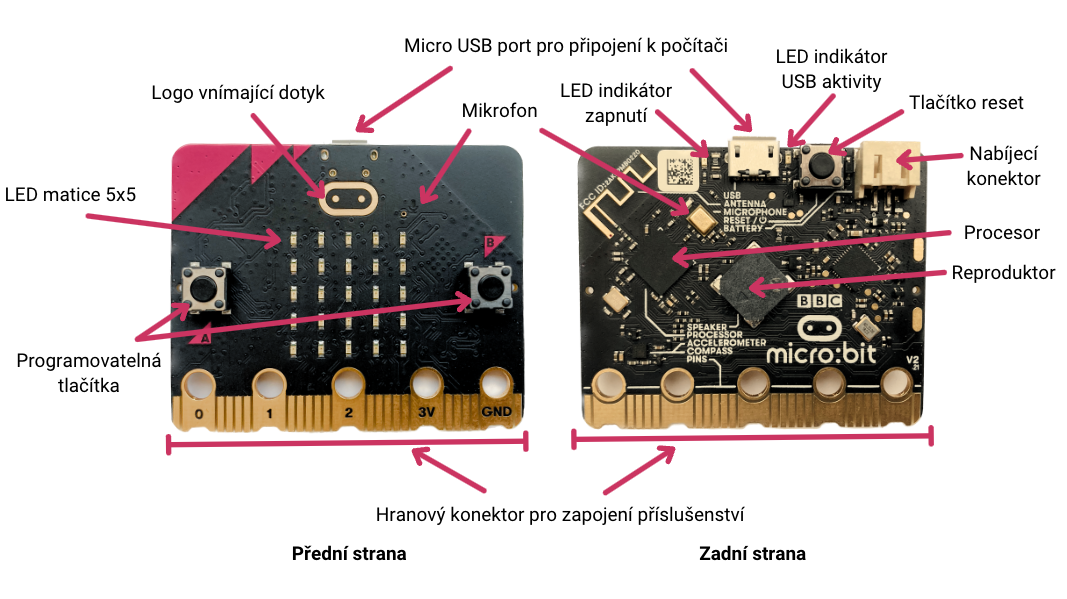
\includegraphics[width=\textwidth] {images/microbit.png}
    \caption{Schéma micro:bitu}
    \label{microbit}
\end{figure}

Micro:bit lze programovat prostřednictvím notebooku, tabletu i~stolního počítače, bez ohledu na operační systém. Ač existují i~editory, které je třeba na zařízení instalovat, mnoho je jich dostupných na internetu. Program se do micro:bitu přenáší pomocí bezdrátové komunikace Bluetooth. Existují tři základní možnosti programování micro:bitu a~to prostřednictvím blokového programování, JavaScriptu a~MicroPythonu. k~dispozici jsou také dva oficiální textové editory, Microsoft MakeCode2 a~MicroPython3.

Výhodou využití robotické stavebnice v~porovnání s~výukou pouze zmíněného Pythonu nebo JavaScriptu je především možnost pochopit princip fungování počítače komplexněji. Programování v~kontextu hardwaru a~nejrůznějších zařízeních založených na senzorech je pro žáky klíčový prvek pro podporování zájmu a~podpoře porozumění ~\cite{Sentance17}. Micro:bit je navržen a~vytvořen primárně s~cílem podpořit výuku informatiky ve školách a~seznámit žáky s~tím, jak mohou počítače řídit různá zařízení. Díky jeho velikosti a~specifickému zaměření odpadá například spouštění plnohodnotného operačního systému a~je možné více pozornosti věnovat informatickému myšlení.

\subsection{Nezha Kit}[ht]
Nezha Inventors Kit je robotická stavebnice navržená pro micro:bit a~je kompatibilní s~první i~druhou verzí. Tato sada pro vynálezce obsahuje několik senzorů PlanetX, díky nimž je možné se sadou vytvořit desítky různých projektů. Základ setu tvoří modul pro umístění micro:bitu. 

\begin{figure}
    \centering
    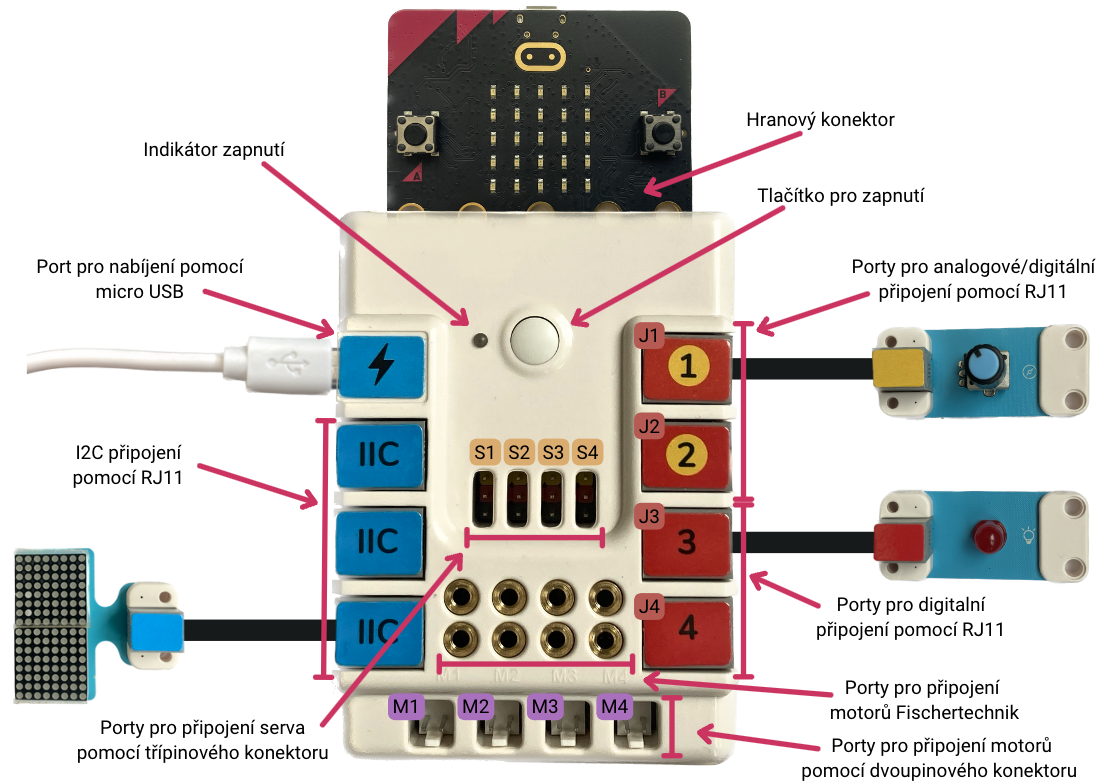
\includegraphics[width=\textwidth] {images/nezha.png}
    \caption{Nezha kit pro micro:bit}
    \label{nezha}
\end{figure}

Pro propojení jednotlivých modulů jsou použity vodiče s~konektory RJ11. Stačí zacvaknout a~senzory jsou propojené s~modulem a~tedy i~s~micro:bitem. Propojení je snadné a~spolehlivé. Další výhodou je kompatibilita Nezha kitu se stavebnicí lego a~fischertechnik. Sada je uložena v~praktickém boxu, který obsahuje:
\begin{itemize}
    \item Nezha rozšiřující modul pro micro:bit (zabudovaný akumulátor LiPol 900 mAh, porty pro senzory a~další moduly, konektory pro serva a~motory, konektor pro micro:bit),
    \item 8 elektronických modulů (3 x LED modul, potenciometr, snímač vlhkosti, snímač vzdálenosti, snímač nárazu, snímač čáry),
    \item 2 x DC motor pro realizaci otáčivých pohybů,
    \item servo 360 ° pro natočení na přesný úhel v~rozsahu 0 -- 360 °,
    \item propojovací vodiče s~konektory RJ11, USB kabel pro nahrání programu do micro:bitu,
    \item kola s~pneumatikami pro LEGO®, rejdovací kolečko pro jezdícího robota,
    \item více než 400 součástí kompatibilních s~LEGO® Technic,
    \item mapa s~čárou pro ježdění po čáře.
\end{itemize}

\begin{figure}
    \centering
    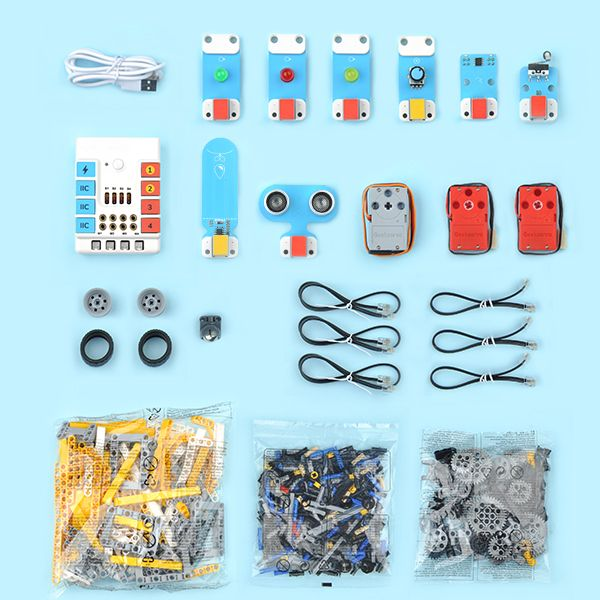
\includegraphics[width=\textwidth] {images/nezhaKit.jpg}
    \caption{Obsah Nezha kitu \cite{nezhasSet}}
    \label{nezhakit}
\end{figure}


\section{Jazyky a~prostředí}
Platforma micro:bit se díky možnosti blokového programování, které je velmi populární pro svou jednoduchost a~uživatelskou přívětivost, hodí pro úplné začátečníky. Zároveň se však neomezuje jen na bloky a~umožňuje jednoduše přejít na Python JavaScript a~případně i~jiné jazyky v~závislosti na zvoleném editoru. 

\subsection{Blokové programování}
Blokové programování je velmi vhodný způsob, jak rozvíjet počítačovou gramotnost již od nízkého věku žáků zvláště pokud cílem není vychovat programátory, ale jedince orientující se v~technologickém světě~\cite{Weintrop19}. Blokové programování poskytuje úvod do strukturovaného programování prostřednictvím barevných bloků, které se přetahují a~spojují do sekvencí. Takto poskládané bloky pak tvoří výsledný program.

Pro práci s~blokovými jazyky je třeba jen, aby žáci uměli číst a~pracovat s~myší. Pro žáky je takový přístup snazší, protože zamezuje chybám v~syntaxi. Žáci můžou více energie věnovat otázce, jak vyřešit problém, což jim umožní si rychleji osvojit algoritmické myšlení. Samotné skládání bloků připomíná puzzle, bloky do sebe zapadnou jen tehdy, není-li porušena syntaxe. Žáci tedy hned ví, že je něco špatně. z~hlediska výuky algoritmizace je výhoda, že se tím žáci zpočátku nemusí zabývat.

\subsubsection{Proměnné a~datové typy}
Protože blokové programování využívá stejné struktury (např. cykly, podmínky, proměnné), jako běžné programovací jazyky, je pro žáky snazší na tomto pochopit princip fungování jednotlivých příkazů. 

Blokové jazyky obvykle však nepracují s~typováním, a~proto, to při přechodu na některý ze silně typovaných jazyků může z~počátku dělat problémy. Bývá deklarován jen číselný datový typ, který se využívá k~uchovávání počtu nějakých jednotek a~následné kontrole např. za účelem ukončení programu. Deklarace proměnné probíhá pouze tak, že se vytvoří v~sekci proměnné, tam se přiřadí pojmenuje a~dále se s~ní pracuje jako s~libovolným jiným blokem.

\subsubsection{Blokové jazyky}
Na základních školách se žáci pravděpodobně již setkali s~některým blokovým jazykem.

Scratch je velmi oblíbený jazyk, který se dodává spolu s~IDE (Integrated Development Envirnoment), které je multiplatformní. IDE je dostupné z~desktopové instalace pro Windows, Mac OS a~Linux, i~jako webová verze, která se po zaregistrování a~přihlášení se do účtu chová jako hub pro uchovávání a~sdílení projektů. Scratch vznikl v~roce 2005 na MIT jako projekt Mitchela Resnicka. a~je poměrně hojně využívaná ve vzdělávání nebo výzkumech.

Dalším zástupcem je Robotanik, robot zahradník. Narozdíl od Scratche nezahrnuje cykly a~větvení.

\subsection{Python}
Python je vysokoúrovňový, interpretovaný programovací jazyk, který nabízí podporu pro různá programovací paradigmata. v~případě micro:bitů si vystačíme s~imperativním. Je dynamicky typovaný a~tedy by žáci po přechodu z~bloků nemuseli mít zásadní problém. Syntaxe je založena na oddělování kódu pomocí bílých znaků, které oddělují jednotlivé bloky a~přispívají k~dobré čitelnosti. Zároveň tento způsob zápisu do jisté míry připomíná práci s~bloky, které zapadají do sebe a~tvoří podobnou strukturu.

Python je zvolen z~mnoha důvodů. Jedním z~nich je jednoduchá syntaxe. Například v~porovnání s~jazyky Java nebo C klade Python důraz na čitelnost a~jednoduchost kódu. Stručná syntaxe jazyka umožňuje vyjadřovat mnohé koncepty v~nižším počtu řádků kódu a~udržovat tak v~kódu přehlednost. i~proto se stále více výzkumníků shoduje, že Python  je vhodný programovací jazyk pro začátečníky~\cite{Wainer18, Narayanan19, Lo15}. Ačkoli se pro výuku programování využívají i~jiné jazyky žáci v~nich obvykle čelí problémům. u~naprostých začátečníků jde často o~potíže se syntaxí. v~Pythonu se žáci z~počátku nemusí zabývat třídami a~dalšími složitějšími konstrukty. První programovací jazyk by měl mít jednoduché vstupní/výstupní příkazy, snadno čitelnou a~konzistentní syntaxi a~být nezávislý~\cite{Lo15}.

\subsection{Python pro micro:bit, IDE}
Výuka programování s~micro:bitem umožňuje začít jednoduchými programy s~rychle viditelnými výsledky. Je však třeba vybrat programovací jazyk tak, aby byl přizpůsoben práci s~micro:bity. z~důvodů zmíněných výše jsou vhodné jazyky založené na Pythonu. v~této kapitole bude provedeno porovnání dvou možností: MicroPython a~MakeCodePython. Na základě srovnání bude vybrán jazyk nejvíce odpovídající požadavkům a v~něm následně řešeny úlohy.

\subsubsection{MicroPython a~vhodné IDE}
Jazyk MicroPython implementuje standard Pythonu 3.4, respektuje jeho syntax a~mnoho funkcí je totožných s~Pythonem, ze kterého vychází. Lze tedy s~výhodou využívat oficiální dokumentaci Pythonu dostupnou z~docs.python.org. MicroPython je zcela kompatibilní s~Pythonem, a~zároveň je optimalizovaný pro běh na mikrocontrolerech, využívá minimální množství zdrojů~\cite{microPython}. Díky této kompatibilitě je možné velmi snadno přenést odladěný kód z~PC na zvolený mikrocontroler nebo vestavěný systém.

\begin{footnotesize}
\begin{lstlisting}[language=Python, caption={MicroPython ukázka}, label={ukazkaMicroPython}]
from microbit import *

for _ in range(2):
    display.show(Image.HEART)
    sleep(1000)
    display.scroll('Hello')
\end{lstlisting}
\end{footnotesize}

Při výběru IDE pro MicroPython a~micro:bit bereme v~úvahu několik faktorů. 
Vzhledem k~již zmíněné kompatibilitě, lze využít jakékoliv IDE pro programování Pythonu. Mezi oblíbené patří Visual Studio Code s~příslušným pluginem nebo Pycharm od JetBrains. Nevýhoda těchto dvou IDE tkví v~jejich komplexitě, která by při výuce a~práci s~micro:bitem byla spíše na škodu. Pro výuku programování by bylo spíše kontraproduktivní využívat software, který má příliš možností a~pro daný účel nadbytečných funkcí. Dále neintegrují funkci přenosu kódu, ta je však nezbytná a~musí být pro žáka jednoduchá.

Zástupci těch méně komplexních editorů vhodných pro vývoj MicroPythonu jsou Mu a~webový editor python.microbit.org. Obě IDE mají tlačítka pro snadný přenos kódu do microbitu, jsou přívětivá pro začínající programátory, snadno se používají a~obě mají sériový výstup. 

\begin{figure}[ht]
    \centering
    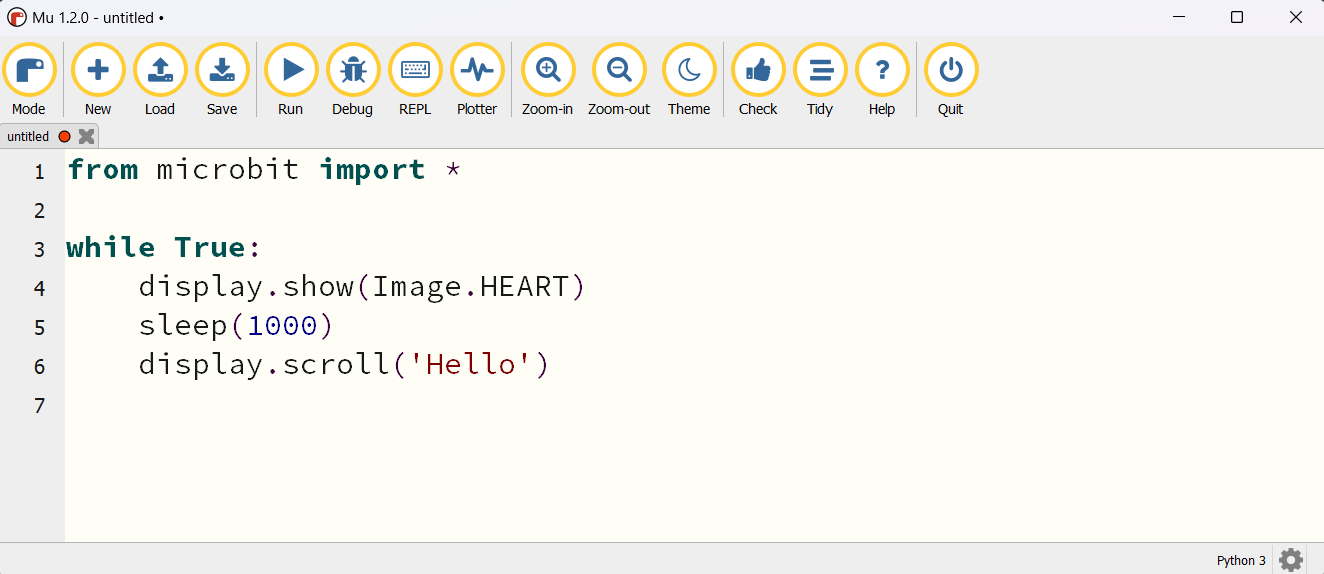
\includegraphics[width=\textwidth]  {images/mu.png}
    \caption{Mu editor}
    \label{MuED}
\end{figure}

Výhodou python.microbit.org oproti Mu jsou hned dvě věci. Jedna z~nich je náhled micro:bitu, ovšem bez modulů. Druhá je panel reference, nebo-li dokumentace, která umožňuje vyhledání kódu, klíčových slov nebo dokonce řídících struktur přímo v~editoru. Navíc je ještě možné tento kód drag\&drop nebo kopírováním přenést do editoru, zeditovat a~ihned použít. 

\begin{figure}[ht]
    \centering
    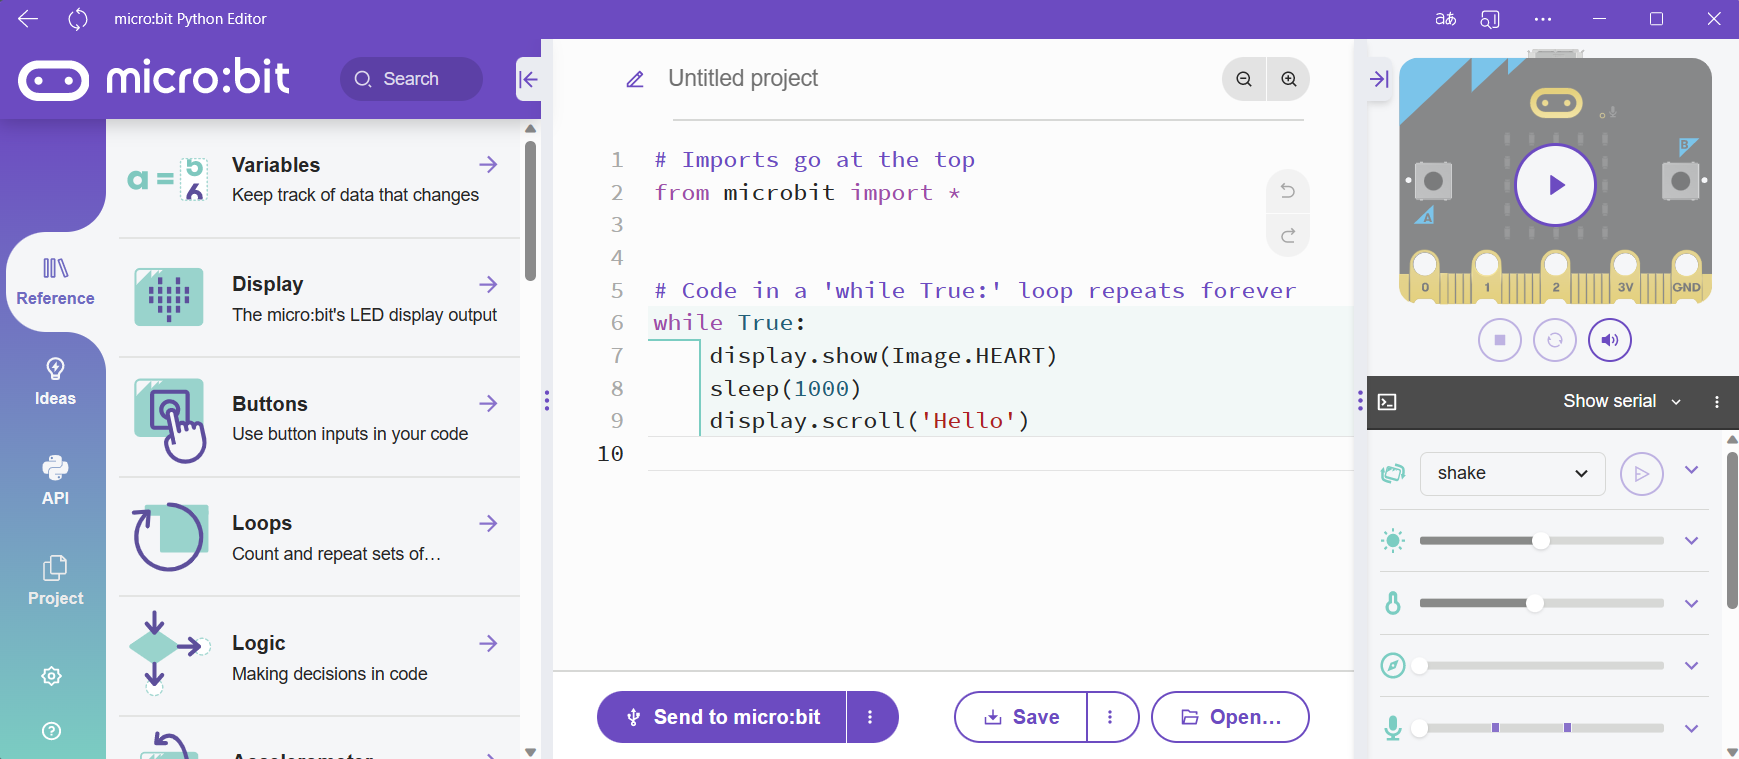
\includegraphics[width=\textwidth]  {images/pythonMBE.png}
    \caption{Python micro:bit editor}
    \label{MicroBitED}
\end{figure}

Významný rozdíl mezi editory je také dostupnost a~údržba IDE. Editor python.microbit.org je webová aplikace, která umožňuje spustit editor odkudkoli, což žákům usnadňuje samostudium. Proti tomu editor Mu je desktopová aplikace, kterou je nutné udržovat. 

Pro účely výuky programování na střední škole je tedy vhodnější python.microbit.org IDE. Jeho použití je snadné, integruje potřebné funkce pro snadné programování micro:bitu.
%\vspace{1cm}

\subsubsection{MakeCode Python, MakeCode IDE}

MakeCode editor umožňuje přímý překlad mezi JavaScriptem, MakeCodePythonem a~bloky. Přímý překlad mezi těmito jazyky způsobuje, že MakeCodePython má určitá omezení proti plnohodnotnému Pythonu. MakeCodePython importuje všechny STS (StaticTypeScript) jmen\-né prostory~\cite{makeCodePython}. Tedy i~malý program, jako např. Hello World, má obrovské množství importů a~přebytečné množství dostupných knihovních funkcí, což snižuje přehlednost nápovědy při psaní programu.

\begin{footnotesize}
\begin{lstlisting}[language=Python, caption=MakeCode Python ukázka]
while True:
    basic.show_icon(IconNames.HEART)
    basic.pause(1000)
    basic.show_string("Hello")
\end{lstlisting}
\end{footnotesize}

Pro MakeCodePython existuje jediné IDE a~to MakeCode IDE. Zde tedy nemáme jinou možnost a~spolu s~výběrem jazyka automaticky vybíráme i~editor. Programování v~MakeCode IDE zpříjemňuje začátečníkům panel s~bloky kódu umístěný vlevo. Bloky lze snadno přetáhnout a~automaticky převést na kód v~Pythonu nebo JavaScriptu, nevýhodou je, nemožnost tento panel zcela skrýt.

\begin{figure}[ht]
    \centering
    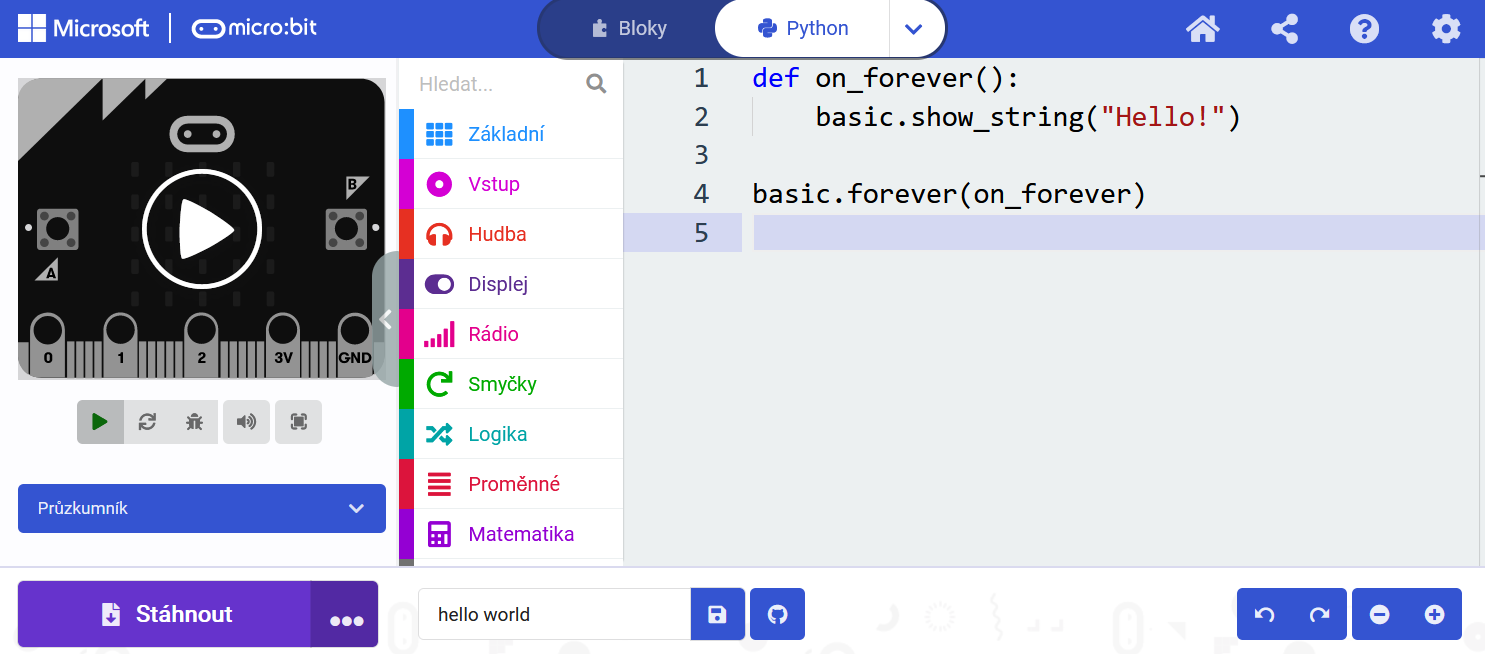
\includegraphics[width=\textwidth]  {images/makecodeE.png}
    \caption{MakeCode editor}
    %\label{fig:my_label}
\end{figure}

\subsubsection{Porovnání možností jazyků a~IDE} 
Oba z~popsaných jazyků umožňují uživatelům programovat micro:bit a~jsou založené na Pythonu. Je mezi nimi však několik rozdílů.

MicroPython vychází z~Pythonu 3 a~je mu tedy mnohem podobnější než MakeCodePython. MicroPython umožňuje využívat v~programu jen knihovny, které jsou aktuálně potřeba, zároveň je možné importovat i~některé z~dalších knnihoven Pythonu 3. Proti tomu MakeCodePython využívá pouze vestavěné funkce, které slouží k~ovládání modulů.

Pro MakeCodePython je dostupný pouze jeden editor, který umí přepínat mezi blokovým programováním a~textovým kódem. Pro MicroPython žádný z~nejpoužívanějších editorů tuto funkci nemá. Pro výuku na středních školách  přepínání není nezbytné, vzhledem k~aktuálnímu RVP se očekává, že žáci se již na základní škole setkali s~blokovým programováním. Nyní je cílem tyto znalosti prohloubit programováním v~textovém editoru.  MicroPython má navíc ve zvoleném python.microbit.org editoru zabudovanou dokumentaci s~možností přetáhnout ukázky Python kódu do vývojového prostředí.

Na základě uvedených aspektů se jako vhodnější jeví MicroPython s~python.microbit.org IDE. z~tohoto důvodu budou v~následujících kapitolách úlohy realizovány prostřednictvím jazyka MicroPython. 

%Využité metody - aplikovat v~konkrétních úlohách?
\chapter{Výukové metody využívané v~lekcích}
Další část práce se zaměřuje na popis konkrétních výukových metod, které jsou implementovány v~metodickém zpracování lekcí. Mezi tyto metody patří například metoda PRIMM, párové programování, Parsons problem a~další. Každá z~těchto metod má své specifické principy a~cíle, které přispívají k~efektivnímu a~interaktivnímu vzdělávání žáků.

\section{PRIMM}
Metoda PRIMM slouží pro strukturování lekcí programování. Pro začínající programátory může být velmi stresující a~nepříjemné začínat psát do prázdného editoru. Když dostanou úvodní část programu od vyučujícího dá se vyvarovat počátečnímu zklamání z~neúspěchu v~případě, že by jejich vlastní kód nefungoval~\cite{hw}.

Metoda se skládá z~pěti částí. 
\begin{itemize}
\item \textit{Predict} -- předvídat, žáci dostanou malou část kódu a~jejich úkolem je zjistit, co bude dělat, když se spustí. 
\item \textit{Run} -- spustit kód a~ověřit předpoklad. Žáci diskutují ve skupinách, zda správně vyhodnotili, jak se bude program chovat. Případně rozeberou v~čem se spletli a~z jakého důvodu. 
\item \textit{Investigate} -- vyučující zadá úkol, pomocí kterého žáci důkladně kód prozkoumají. 
\item \textit{Modify} -- žáci upravují program, mění nebo přidávají funkcionalitu dle zadání. Využívají, že v~předchozích částech pochopili strukturu kódu. Žák překlene hranici z~cizího kódu k~částečně vlastnímu. 
\item \textit{Make} -- žáci vytvoří nový program, který využívá stejné struktury a~koncepty, jako předchozí, ale řeší jiný problém. v~posledním kroku již tedy žáci píší vlastní program.
\end{itemize}

\section{Koncept převrácené třídy}
Koncept převrácené třídy, v~angličtině označováno \textit{flipped classrooms} je způsob výuky, který vede žáky k~odpovědnosti za své studium a~výsledky. 
Žáci dostanou předem materiály a~zdroje sloužící k~samostudiu a~samotné hodiny slouží spíše pro praktické úkoly, či jako prostor pro konzultace. Vyučující se pak může více zaměřit na individuální potřeby každého žáka a~poskytovat jim individuální pomoc a~zpětnou vazbu.
Tento koncept má několik výhod. Je flexibilní, žáci mají na studium tolik času, kolik potřebují a~mohou se učit v~době, která jim vyhovuje. Šetří se čas, není třeba předávat informace, které jsou jednoduše dostupné~\cite{mazur09}. Zároveň však hned na úvod vznikají rozdíly mezi těmi žáky, kteří se tématu předem věnovali a~těmi, kteří z~jakéhokoli důvodu ne.

\section{Párové programování}
Pedagogický přístup, zahrnující dva žáky pracující spolu na problému, který je třeba vyřešit. Jsou rozděleny role. Jeden z~žáků ovládá klávesnici a~myš, soustředí se na drobné kroky, které má před sebou a~aktuálně neřeší větší problémy. Druhý žák je v~roli pozorovatele a~navigátora, kontroluje kód, v~případě nejasností nebo pochybností je sdílí. Zároveň si udržuje přehled o~struktuře a~celistvosti kódu.

Je důležité, aby si žáci role pravidelně střídaly, jen tak se zajistí stejnoměrné zapojení obou aktérů~\cite{Hanks11}. Mezi partnery jsou neustále předávány znalosti, ale i~zkušenosti a~návyky. Je obvyklou praxí vytvářet páry nevyvážené, kdy jeden z~dvojice je pokročilejší, než druhý. v~praxi je tento systém běžně využíván v~softwarových firmách při vývoji.

\section{Code review}
Vzájemné hodnocení kódu je proces založený na sdílení kódu s~další osobou, jejíž úkolem je dát zpětnou vazbu. Vzájemné hodnocení je uznáváno jako pedagogicky cenné protože žáky může naučit poskytovat konstruktivní zpětnou vazbu ostatním a~zároveň je připravit na zvládání kritiky. Žáci, kteří si psali vzájemné hodnocení dosahovali lepších výsledků než ti, kteří tak nečinili~\cite{Hundhausen13}. Po obdržení hodnocení mají žáci obvykle možnost upravit své řešení na základě zpětné vazby a~znovu jej předat k~posouzení. Tím, že je po žácích vyžadováno, aby zkoumali kód ostatních a~vyjádřili se k~němu se zlepšuje jejich schopnost orientovat se v~programu, který napsal někdo jiný. 

\section{Hledání vlastních chyb}
Jedna z~účinných technik pro výuku hledání vlastních chyb je záměrné rozbíjení kódu a~pozorování výsledků~\cite{Love22}. Pro začátek žákům poskytněte soubor kódu v~jazyce Python. Poté je instruujte, aby systematicky odstraňovali části kódu a~tím vytvářeli běžné chyby. Po spuštění programu okamžitě obdrží zpětnou vazbu, která jim pomůže vytvořit spojení mezi chybami, chybovými zprávami a~řešením problému. Tímto způsobem studenti zlepšují své dovednosti v~ladění kódu.

Další možná metoda je naučit žáky po napsání každé drobné části kódu program spustit a~zkontrolovat, že je možné ho bez chyb spustit. Tato metoda ušetří čas, který by později bylo nutné věnovat hledání chyb. Zvláště v~netypovaných jazycích, lze touto metodou zabránit nevhodné práci s~proměnnými.

\section{Parsons problem}
Parsons problem je metoda založená na principu skládání již připravených bloků nebo řádků kódu do správného pořadí. Výhodou je například soustředění se na bloky kódu a~algoritmus namísto řešení problémů se syntaxí, které je v~počátku pro mnohé odrazující. Některé takové skládačky mohou obsahovat řádky nebo bloky kódu, které jsou navíc a~je potřeba je vynechat. Použití těchto \textit{distractors} se však ukazuje jako kontraproduktivní~\cite{Harms16}. Nemá žádný pozitivní přínos a~zároveň snižují efektivitu učení.

\chapter{Metodické zpracování úloh}
Obsahem této části práce jsou řešené úlohy, doplněné o~metodické pokyny pro učitele. Cílem bylo vytvořit úlohy tak, aby byly pro žáky zajímavé a~praktické. Díky využití micro:bit kitu je možné programovat fyzické komponenty, které se chovají dle toho, jak je žáci naprogramují. Zadání mají za cíl naplnit požadavky revidovaného RVP, jež je popsáno v~předchozích kapitolách. Příklady i~jejich řešení obsahují metodické poznámky, aby i~učitel, který nemá přehled v~dané oblasti měl všechny potřebné informace a~mohl žáky bez obtíží provést úlohou. Při tvorbě struktury jsem vycházela z~učebnice Python3~\cite{Summerfield10}.

\section{Struktura materiálu a~obecná doporučení}
Úlohy jsou koncipované tak, aby byly interaktivní a~umožnily žákům v~reálném čase vidět, jak jejich kód funguje, což je velmi užitečné pro porozumění a~probuzení zájmu o~programování~\cite{Fagerlund22}. 

Tento materiál je navrhnut na deset lekcí, které obsahují příklady uspořádané dle náročnosti vytvořené na základě požadavků kladených ze strany RVP G. Rozvržení lekcí bylo inspirováno prostudovanými materiály, především učebnicí Robotika pro střední školy: programujeme Micro:Bit pomocí Pythonu, která je schválena MŠMT~\cite{pythonImysleni}. Pořadí lekcí vychází z~učebnice Python 3: výukový kurz~\cite{Summerfield10} a je následující: 
\vspace{0,1cm}
\begin{compactitem}
    \item[0.] Seznámení s materiálem
    \item[1.] Úvod do algoritmizace a první program
    \item[2.] Proměnné a datové typy
    \item[3.] Větvení, podmínky a logické operátory
    \item[4.] While cyklus
    \item[5.] For cyklus
    \item[6.] Seznamy, indexace, foreach
    \item[7.] Funkce a metody
    \item[8.] Testování
    \item[9.] OOP a moduly
    \item[10.] Projekt
\end{compactitem}
\vspace{0,1cm}
Lekce začínají seznámením s tvorbou a spouštěním programu na klasické úloze \textit{Hello World}. Následuje představení datových typů, řídících struktur a funkcí. Zařazena dříve byla 8. lekce, jejiž náplní je otestovat a opravit cizí program. Zařazena byla tato lekce tak, aby žáci již znali dostatek konceptů pro možnost testování komplexnějšího programu skládajícího se z~funkcí a~zároveň nenastala situace, že v~průběhu školního roku se tato kapitola nestihne. Následuje úvod do objektově orientovaného programování a seznámení s moduly. Závěrečná lekce je věnována projektu, na kterém žáci prokáží, získané znalosti.

\subsection{Struktura výukového materiálu} 
Materiály jsou dostupné na \href{https://github.com/denisa-mat/BP-microbit}{GitHubu}, kde jsou umístěny všechny lekce, zadání příkladů včetně potřebných modulů i~zdrojové kódy s~jejich ukázkovým řešením. Materiál obsahuje deset lekcí, z~nichž každá je koncipována pro dvě vyučovací hodiny ideálně následující hned po sobě. v~lekcích je dohromady XXX % END
úloh, ve kterých žáci pracují s~micro:bitem a v~editoru python.microbit.org programují v~MicroPythonu.

Struktura repozitáře na \href{https://github.com/denisa-mat/BP-microbit}{GitHubu} je následující. Každá kapitola má vlastní větev, v~níž jsou umístěny následující soubory:
\vspace{0,1cm}
\begin{compactitem}
    \item readme.md obsahující kompletní strukturu lekce,
    \item XX\_exercises.py se zadáním a vzorovou implementací úloh
    \item složka s moduly využitými v dané lekci
\end{compactitem}

Lekce začínají uvedením cíle a~motivací žáků. Cílem je žáky motivovat, dodat jim energii k~přemýšlení a~soustředění~\cite{Filgona20}. Ukázat jim, jak lze dovednosti, které se naučí, prakticky využít. Nelze předpokládat, že si žáci uvědomují důležitost lekcí. Je třeba ukázat přínos pro jejich potřeby.

Poté následuje teoretická část, kde jsou žákům představeny základní prostředky, teorie, syntax programovacího jazyka a~další teoretická východiska, které jsou potřebné pro řešení konkrétních problémů v~dané lekci. Účelem je žákům dané koncepty vysvětlit jednoduše a~srozumitelně. Stále je však kladen důraz na exaktnost předávané teorie. Snažíme se, aby tato část nebyla pouze frontálním výkladem učitele, proto má v~lekcích různé podoby. 

Po teoretické části žáci dostanou konkrétní úkol nebo problém, který bude jejich úkolem vyřešit. Při zadávání úkolů je důležité, aby byly jasně definované a~žákům bylo jasné, co se od nich očekává.  i~zde existuje mnoho způsobů, jak lze dosáhnout praktického vyzkoušení a~osvojení teoretických konceptů, které jim byly představeny v~předchozí části. Žáci mohou pracovat na řešení daného problému samostatně nebo ve skupinách. Vyučující v~této fázi působí především jako průvodce, je k~dispozici a v~případě potřeby žákům nabízí pomoc. Učitel by také měl být schopen rozlišit, kdy poskytnout pomoc a~kdy nechat žáky řešit problémy samostatně. Některé lekce jsou založené na jediném větším úkolu, jinde je více menších.

Na závěr lekce přichází krátké shrnutí doplněné o~několik otázek sloužících k~ověření znalostí. Smyslem je, aby si žáci uvědomili, co bylo pro vyřešení úkolu nejdůležitější a~jak to mohou využít při řešení obdobných problémů.

Poslední odstavec obsahuje doplňující poznámky pro učitele, které se vztahují obecně k~celé lekci, obsahuje například odkazy na rozšiřující zdroje.  %TODO přepsat odstavec

\section{Zpracování lekcí}

Tato kapitola se věnuje samotné realizaci lekcí a k nim vytvořeným úlohám. Popsány zde budou pouze vybrané z nich. %TODO - vybrané jak?
Celý materiál je možné najít v příloze této práce v archivu %TODO - název archivu
a také ve veřejném repozitáři na \href{https://github.com/denisa-mat/BP-microbit}{GitHubu}. Materiál je zveřejněn pod licencí CC BY 3.0 CZ a je možné jej volně využívat a upravovat.

\subsection{Lekce 0 -- Seznámení s materiálem}
Nultá lekce slouží učitelům k~seznámení se strukturou tohoto materiálu a~vyjasnění některých záležitostí hned v~úvodu. Cílem materiálu je přiblížit žákům algoritmizaci a~programování bez předchozí znalosti Pythonu. 

Obsah lekcí je sestaven tak, aby odpovídal požadavkům plynoucím z~revidovaného RVP. Žáci by na konci měli znát základní programové řídící struktury. Budou schopni vytvořit a~zapsat algoritmus řešící zadaný problém a~na základě něho vytvoří program v~jazyce Python využívající cykly, větvení, proměnné a~seznamy. Žáci dokáží program dekomponovat na funkce s~parametry a~návratovými hodnotami.

Praktické úlohy jsou realizovány pomocí MicroPythonu a~sady Nezha pro micro:bit, je zde tedy specifikováno jaké nástroje jsou pro práci s~materiálem potřeba. Dále je uvedena časová náročnost, která odpovídá deseti blokům výuky. Každý blok na dvě vyučovací hodiny.

Následuje popis struktury vzniklého materiálu, který je v~této práci popsán v~kapitole 5.1.1. v~závěru je stručně popsána struktura a~klíčové prvky jednoduchého programu v~MicroPythonu. 
\begin{footnotesize}
\begin{lstlisting}[language=Python, caption=struktura programu v~MicroPythonu]
from microbit import *

# Nasleduje nekonecny cyklus

while True:
    display.scroll("Hello World")
\end{lstlisting}
\end{footnotesize}

Na prvním řádku je import knihovny microbit, která obsahuje všechny funkce a~metody potřebné pro práci s~micro:bitem. Tento řádek uvozuje všechny vzorové implementace. v~případě, kdy úloha obsahuje práci se senzory, následuje import dalších modulů. Hvězdička značí, že příkaz importuje vše, co knihovna obsahuje.

Znak \# na začátku třetího řádku značí jednořádkový komentář. Komentáře nejsou součástí vykonávaného programu, slouží programátorům pro poznámky týkající se kódu.

Syntaxe Pythonu používá k~identifikaci zanoření odsazení pomocí daného počtu mezer/tabulátoru (v závislosti na IDE). Každý příkaz, který je zanořen je součástí kódu, který je o~úroveň výše.

\subsection{Lekce 1 -- Seznámení s~micro:bitem, IDE a~první program}
První vytvořený program při výuce programovacích jazyků bývá nejčastěji Hello World, jde o~krátký program, který obsahuje pouze zápis příkazu, který vypíše text \textit{Hello World} (česky Ahoj světe)~\cite{helloWorld}. Tento koncept využijeme i~zde v~první lekci pro seznámení s~prostředím a~využívanými nástroji.
\subsubsection{Obsah lekce}
\begin{itemize}
    \item Motivace -- Proč potřebují žáci umět programovat? Ukážeme příklad s~velkým množstvím fotografií, které potřebujeme přejmenovat. Ručně by zabralo velké množství času, vytvoření skriptu může zabrat pár minut práce.
    \item Prostředky -- v~první kapitole je tato část z~větší části teoretická. Je potřeba s~žáky probrat s~čím se bude ve zbytku lekcí pracovat. Představení MicroPythonu jako programovacího jazyka. Popis algoritmu a~jeho vlastností spolu s~ukázkou vývojových diagramů. Představení micro:bitu a~IDE ve kterém se bude micro:bit programovat. 
    \item Shrnutí -- TODO
    \begin{itemize}
        \item ?
        \item ?
        \item ?
    \end{itemize}
    \item Poznámky pro učitele -- v~první lekci zůstane žákům zatajena existence tříd, objektů a~metod, těm se budou věnovat pozdější lekce, zatím se obejdeme bez nich.
\end{itemize}
\subsubsection{Úloha 1 -- Hello World}
\begin{itemize}
    \item Zadání

Napište program, který na vestavěný displej vypíše řetězec Hello World. Následně program nahrajte do micro:bitu.
    \item Co budete potřebovat

K této úloze nejsou potřebné žádné senzory ani Nezha sada.
    \item Co se naučíte

Cílem úlohy je především vytvoření prvního programu v~MicroPythonu. Dále prakticky seznámit žáky s~IDE a~micro:bitem a~program nahrát z~počítače do micro:bitu.
    \item Vzorová implementace
\begin{footnotesize}
\begin{lstlisting}[language=Python, caption=Úloha 1 - Hello World]
from microbit import *

while True:
    display.scroll('Hello World')
\end{lstlisting}
\end{footnotesize}
    \item Popis řešení

Na prvním řádku jsou je z~modulu microbit importováno vše, co obsahuje. v~tomto konkrétním případě lze import celého obsahu nahradit pouze importem objektu display, který pro tuto úlohu stačí. Protože se celý řetězec na maticový displej micro:bitu nevejde, využijte metodu scroll na objektu display, které předáte jako parametr požadovaný textový řetězec "Hello World". Pro opětovná zobrazení bez nutnosti restartování programu obalte příkaz do nekonečného while cyklu.

\begin{figure}[ht]
    \centering
    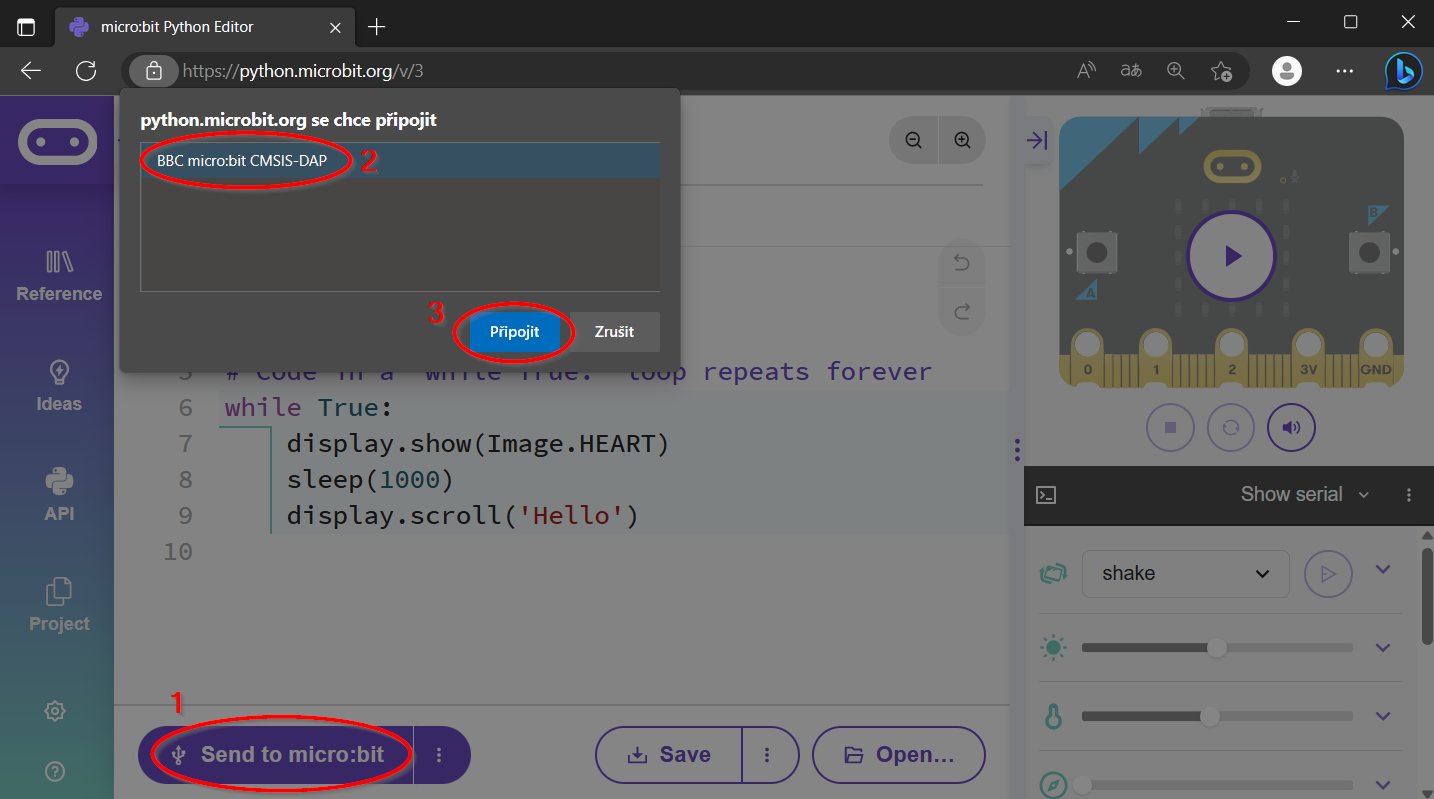
\includegraphics[width=\textwidth]  {images/send1.png}
    \caption{Jak připojit micro:bit}
    %\label{fig:my_label}
\end{figure}

\begin{figure}[ht]
    \centering
    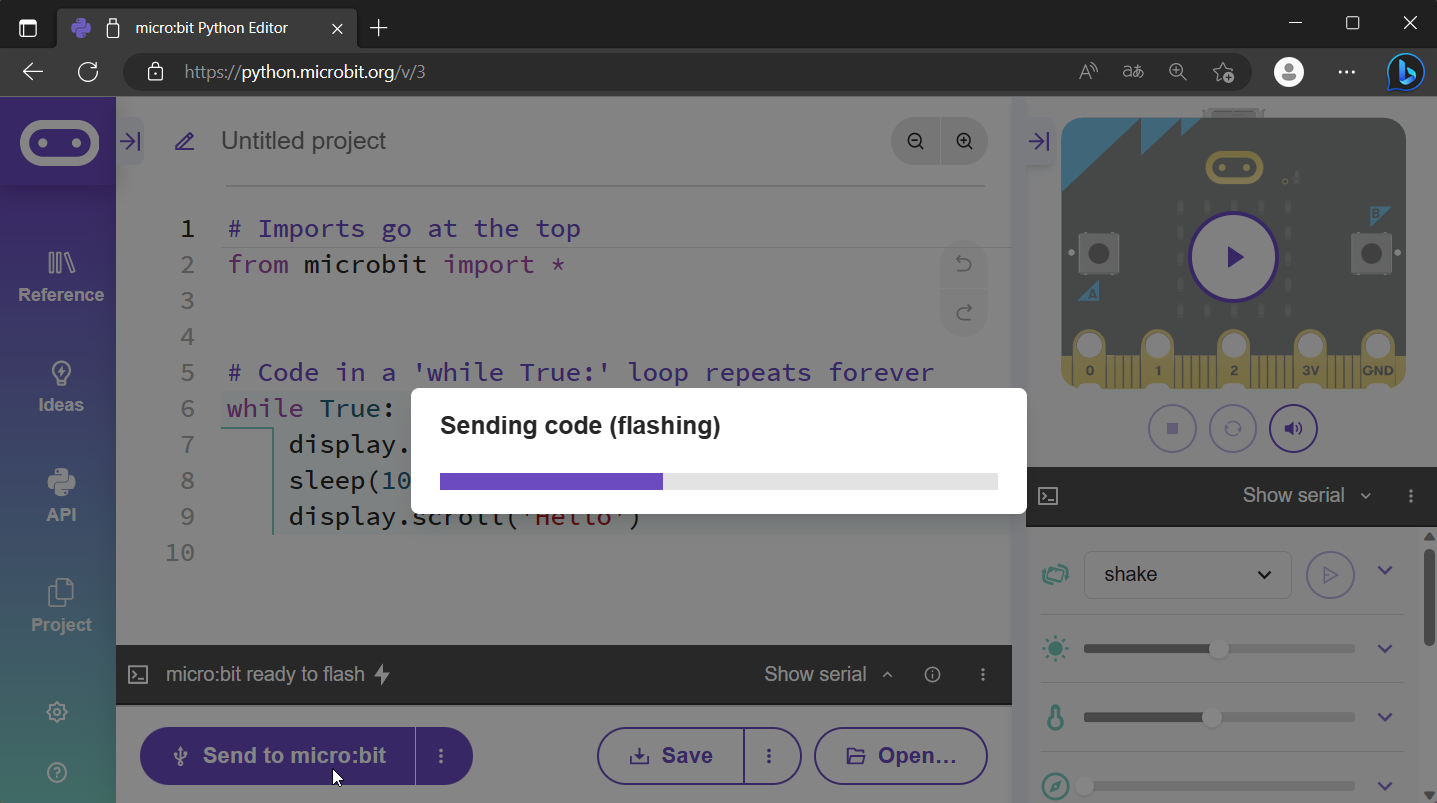
\includegraphics[width=\textwidth]  {images/send2.png}
    \caption{Jak nahrát program}
    %\label{fig:my_label}
\end{figure}

Do micro:bitu program z~počítače nahrajte pomocí přiloženého micro USB kabelu. Ve spodní části obrazovky vyberte "Send to micro:bit", otevře se nápověda a~poté okno s~kompatibilními zařízeními.

Vyberte micro:bit a~klikněte na připojit, zobrazí se progress bar a~program se nahraje do micro:bitu. Ve spodní části obrazovky uvidíte zprávu o~tom, zda se podařilo. Nyní až do odpojení micro:bita stačí pro nové nahrání vždy jen kliknout na tlačítko "Send to micro:bit".

V případě, že tento postup nefunguje je možné program stáhnout ve formátu .hex a~nahrát na micro:bit jako na externí úložiště.

    \item Doplňující poznámky

Cykly budou žákům podrobněji vysvětleny až v~lekci 4, do té doby si vystačíme s~while True, pro neustálé opakování programu. v~případě zájmu si můžou žáci World nahradit svým jménem.
\end{itemize}

\subsection{Lekce 2 -- Proměnné a~datové typy}

\subsection{Lekce 3 -- }

\section{Možnosti rozšíření}
Senzor pro RFID, sledování vlhkosti apod. -- umožňuje dále sbírat data, následná možnost využít v~tématické oblasti týkající se práce s~daty a~jejich zpracování. Zároveň široká škála možností využít v~ostatních přírodovědných předmětech.

Micro:bit je možné vyměnit za Pico:ed, který poskytuje podporu pro jazyk C, zároveň je stále kompatibilní s~Nezha modulem. 

\chapter{Vyhodnocení potřeb}
Vytvořený materiál byl před dokončením konzultován se čtyřmi středoškolskými učiteli informatiky, kteří jsou hlavní skupinou, pro kterou je materiál tvořen. Délka praxe i~zkušenost s~výukou programování se u~jednotlivých učitelů různila, díky tomu se mi podařilo získat velmi cennou zpětnou vazbu a~důležité poznatky týkající se reálné použitelnosti v~hodinách informatiky na středních školách.

\section{Zhodnocení učiteli}
Cílem konzultací bylo zjistit míru skutečné použitelnosti a~identifikovat možnosti dalšího vylepšení. Mezi učiteli nejprve panovaly obavy z~toho, do jaké míry je micro:bit na středních školách skutečně využitelný. Zprvu se někteří domnívali, že k~programování chci využívat bloky, po objasnění skutečnosti obavy opadly.

Učitelé informatiky, s~nimiž jsi měla schůzky, ocenili, že výukový materiál obsahuje nultou lekci s~úvodními informacemi a~speciálně uvedení doporučeného prohlížeče a~editoru. v~jiných materiálech se často setkávají s~tím, že není uveden například operační systém nebo právě prohlížeč a~následně se program chová jinak než je popsáno. 

Dalším pozitivním prvkem jsou popsané vzorové implementace, které umožňují učitelům nahlédnout do toho, jak by mohl program vypadat a~co by mohlo být špatně v~případě, že jim něco nefunguje. Učitelé by byli rádi, kdyby i~vzorových implementací byli řádky programu očíslované i~vzhledem k~tomu, že v~popisu implementace se na konkrétní řádky odkazuji Tento problém jsem řešila, bohužel se mi nepodařilo na GitHubu, kde jsou materiály k~dispozici tuto funkci přidat. Dále by se učitelům líbilo, kdyby byl k~dispozici i~obrazově znázorněný výstup, který ukazuje, jak daný kód funguje v~praxi.

Text samotný byl hodnocen jako srozumitelný a~vhodný pro začátečníky. Zvláště pozitivně hodnotili  popisnost obrázkových návodů. u~některých úloh by především začínající učitelé ocenili detailnější popis, řešení úlohy. Naopak zkušenější učitelé považovali některé popisy za zbytečně podrobné.

Ke koncepci a~návaznosti lekcí učitelé neměli žádné námitky. Pouze navrhují, aby bylo na začátku každé lekce uvedeno, co bude pro danou lekci potřebovat a~mohli si vše jednoduše na lekci připravit. Někteří učitelé měli obavu, zda se lekce během 90 minut stihne, sami však uznali, že je to velmi těžké odhadnout a~záleží od typu školy, ale i~šikovnosti konkrétní třídy.  Učitelé také zmiňovali, že ne vždy mají hodiny informatiky spojené do jednoho bloku a~tak by ocenili, kdyby v~materiálu bylo označeno, kde lze lekci rozdělit. 

Učitelé celkově hodnotili materiál jako kvalitní a~vhodný pro výuku na středních školách především na školách s~obecným vzděláním, nebo školách s~jiným zaměřením než jsou informační technologie.

\section{Možnosti budoucího vylepšení}
Na základě zpětné vazby lze provést několik vylepšení. v~první řadě k~vzorovým implementacím přidat číslování řádků, což umožní učitelům snadno odkazovat na konkrétní řádky programu při vysvětlování nebo řešení problémů. Dále lze doplnit obrazové a~video ukázky zobrazující očekávaný výstup programu. To poskytne žákům lepší představu o~tom, jak kód funguje v~praxi, a~pomůže jim lépe pochopit požadovaný výstup.

Bylo by vhodné uvést informace o~tom, kde je možné lekci rozdělit, aby se lépe přizpůsobila různým školním rozvrhům. Například uvést, že první polovina lekce se zaměřuje na úvod a~teorii, zatímco druhá polovina se věnuje praktickým cvičením a~programování.

Nyní je materiál dostupný pod licencí CC BY 3.0 CZ (Creative commons Uveďte původ 3.0 Česká republika) ve veřejném repozitáři na \href{https://github.com/denisa-mat/BP-microbit/tree/lekce-00}{GitHubu}. Do budoucna by mohlo být přínosné vytvoření webové aplikace, kde by bylo vše pohodlně dostupné. Lze také vytvořit pracovní listy, zadání a~kostry úloh pro žáky, aktuální materiál je určen primárně pro učitele.

Na základě zpětné vazby během využívání materiálů, lze vytvořit odpovědi a~otázky na často se vyskytující problémy a~chyby.

Je důležité si uvědomit, že tato práce není konečným řešením, ale spíše prvním krokem ke zlepšení výuky algoritmizace na středních školách. Existuje potenciál pro další rozšíření sadou úloh, implementaci dalších výukových metod a~využití dalších technologií. Důkladné monitorování a~hodnocení využití platformy micro:bit ve výuce a~průběžná aktualizace výukových materiálů jsou klíčové pro udržení jejich relevance a~efektivity.

\chapter{Závěr}
Tato práce představila platformu micro:bit jako prostředek pro výuku algoritmizace na středních školách v~kontextu revidovaného rámcového vzdělávacího programu pro gymnázia pro oblast informatiky (RVP G). Cílem bylo vytvořit a~zrealizovat sadu úloh, které by pomohly žákům osvojit si základní programovací koncepty a~návrh algoritmů s~využitím programovacího jazyka MicroPython.

V průběhu práce byla provedena analýza současného stavu výuky informatiky na středních školách a~zhodnocení existujících řešení a~materiálů dostupných pro učitele. Na základě získaných znalostí bylo navrženo deset kompletních lekcí, které pokrývají klíčové oblasti algoritmizace a~programování podle revidovaného RVP G. Tyto lekce byly doplněny metodickými pokyny, které učitelům pomohou připravit se na výuku a~efektivně provést žáky jednotlivými tématy.

Došlo k~představení nástrojů a~výukových metod, které jsou využívány jako prostředky při řešení úloh. Mezi tyto nástroje patří robotická stavebnice, micro:bit v~kombinaci s~Nezha kitem, programovací jazyk Python a~MicroPython a~jejich IDE.

Sada úloh zahrnuje různé praktické projekty, ve kterých žáci mohou využít hardware micro:bitu spolu s~programovacím jazykem MicroPython. Úlohy se zaměřují na interaktivní a~experimentální přístup, který umožňuje žákům aktivně se zapojit do procesu učení a~rozvíjet své programovací dovednosti. Důraz byl kladen na základní programovací koncepty, jako jsou podmínky, cykly, proměnné a~funkce, a~jejich aplikaci při návrhu algoritmů.

Důležitým aspektem této práce byla také zpětná vazba od učitelů na vytvořené úlohy. Jejich názory a~hodnocení přispěly k~ vylepšení vytvořených lekcí a~úpravě metodických pokynů. 

\printbibliography[heading=bibintoc] %% Print the bibliography.

  \makeatletter\thesis@blocks@clear\makeatother
  \phantomsection %% Print the index and insert it into the
  \addcontentsline{toc}{chapter}{\indexname} %% table of contents.
  \printindex

\appendix %% Start the appendices.
\chapter{Elektronické přílohy}
Here you can insert the appendices of your thesis.

\end{document}
